\documentclass[11pt]{beamer}
\usetheme{Berkeley}
\usepackage[utf8]{inputenc}
\usepackage[italian]{babel}
\usepackage{amsmath}
\usepackage{amsfonts}
\usepackage{amssymb}
\usepackage{graphicx}
\usepackage{cool}
\usepackage{commath}

\author{Jacopo Tissino}
\title{Turbolenza\\
Fluidodinamica e Van Gogh}
%\setbeamercovered{transparent} 
%\setbeamertemplate{navigation symbols}{} 
%\logo{} 
\institute{Liceo Scientifico ``M. Grigoletti''} 
%\date{} 
%\subject{} 
\begin{document}

\begin{frame}
\titlepage
\end{frame}

\begin{frame}
\tableofcontents
\end{frame}

\section{La turbolenza nei quadri di Van Gogh}

\begin{frame}{\emph{Notte Stellata}}
\begin{figure}
\centering
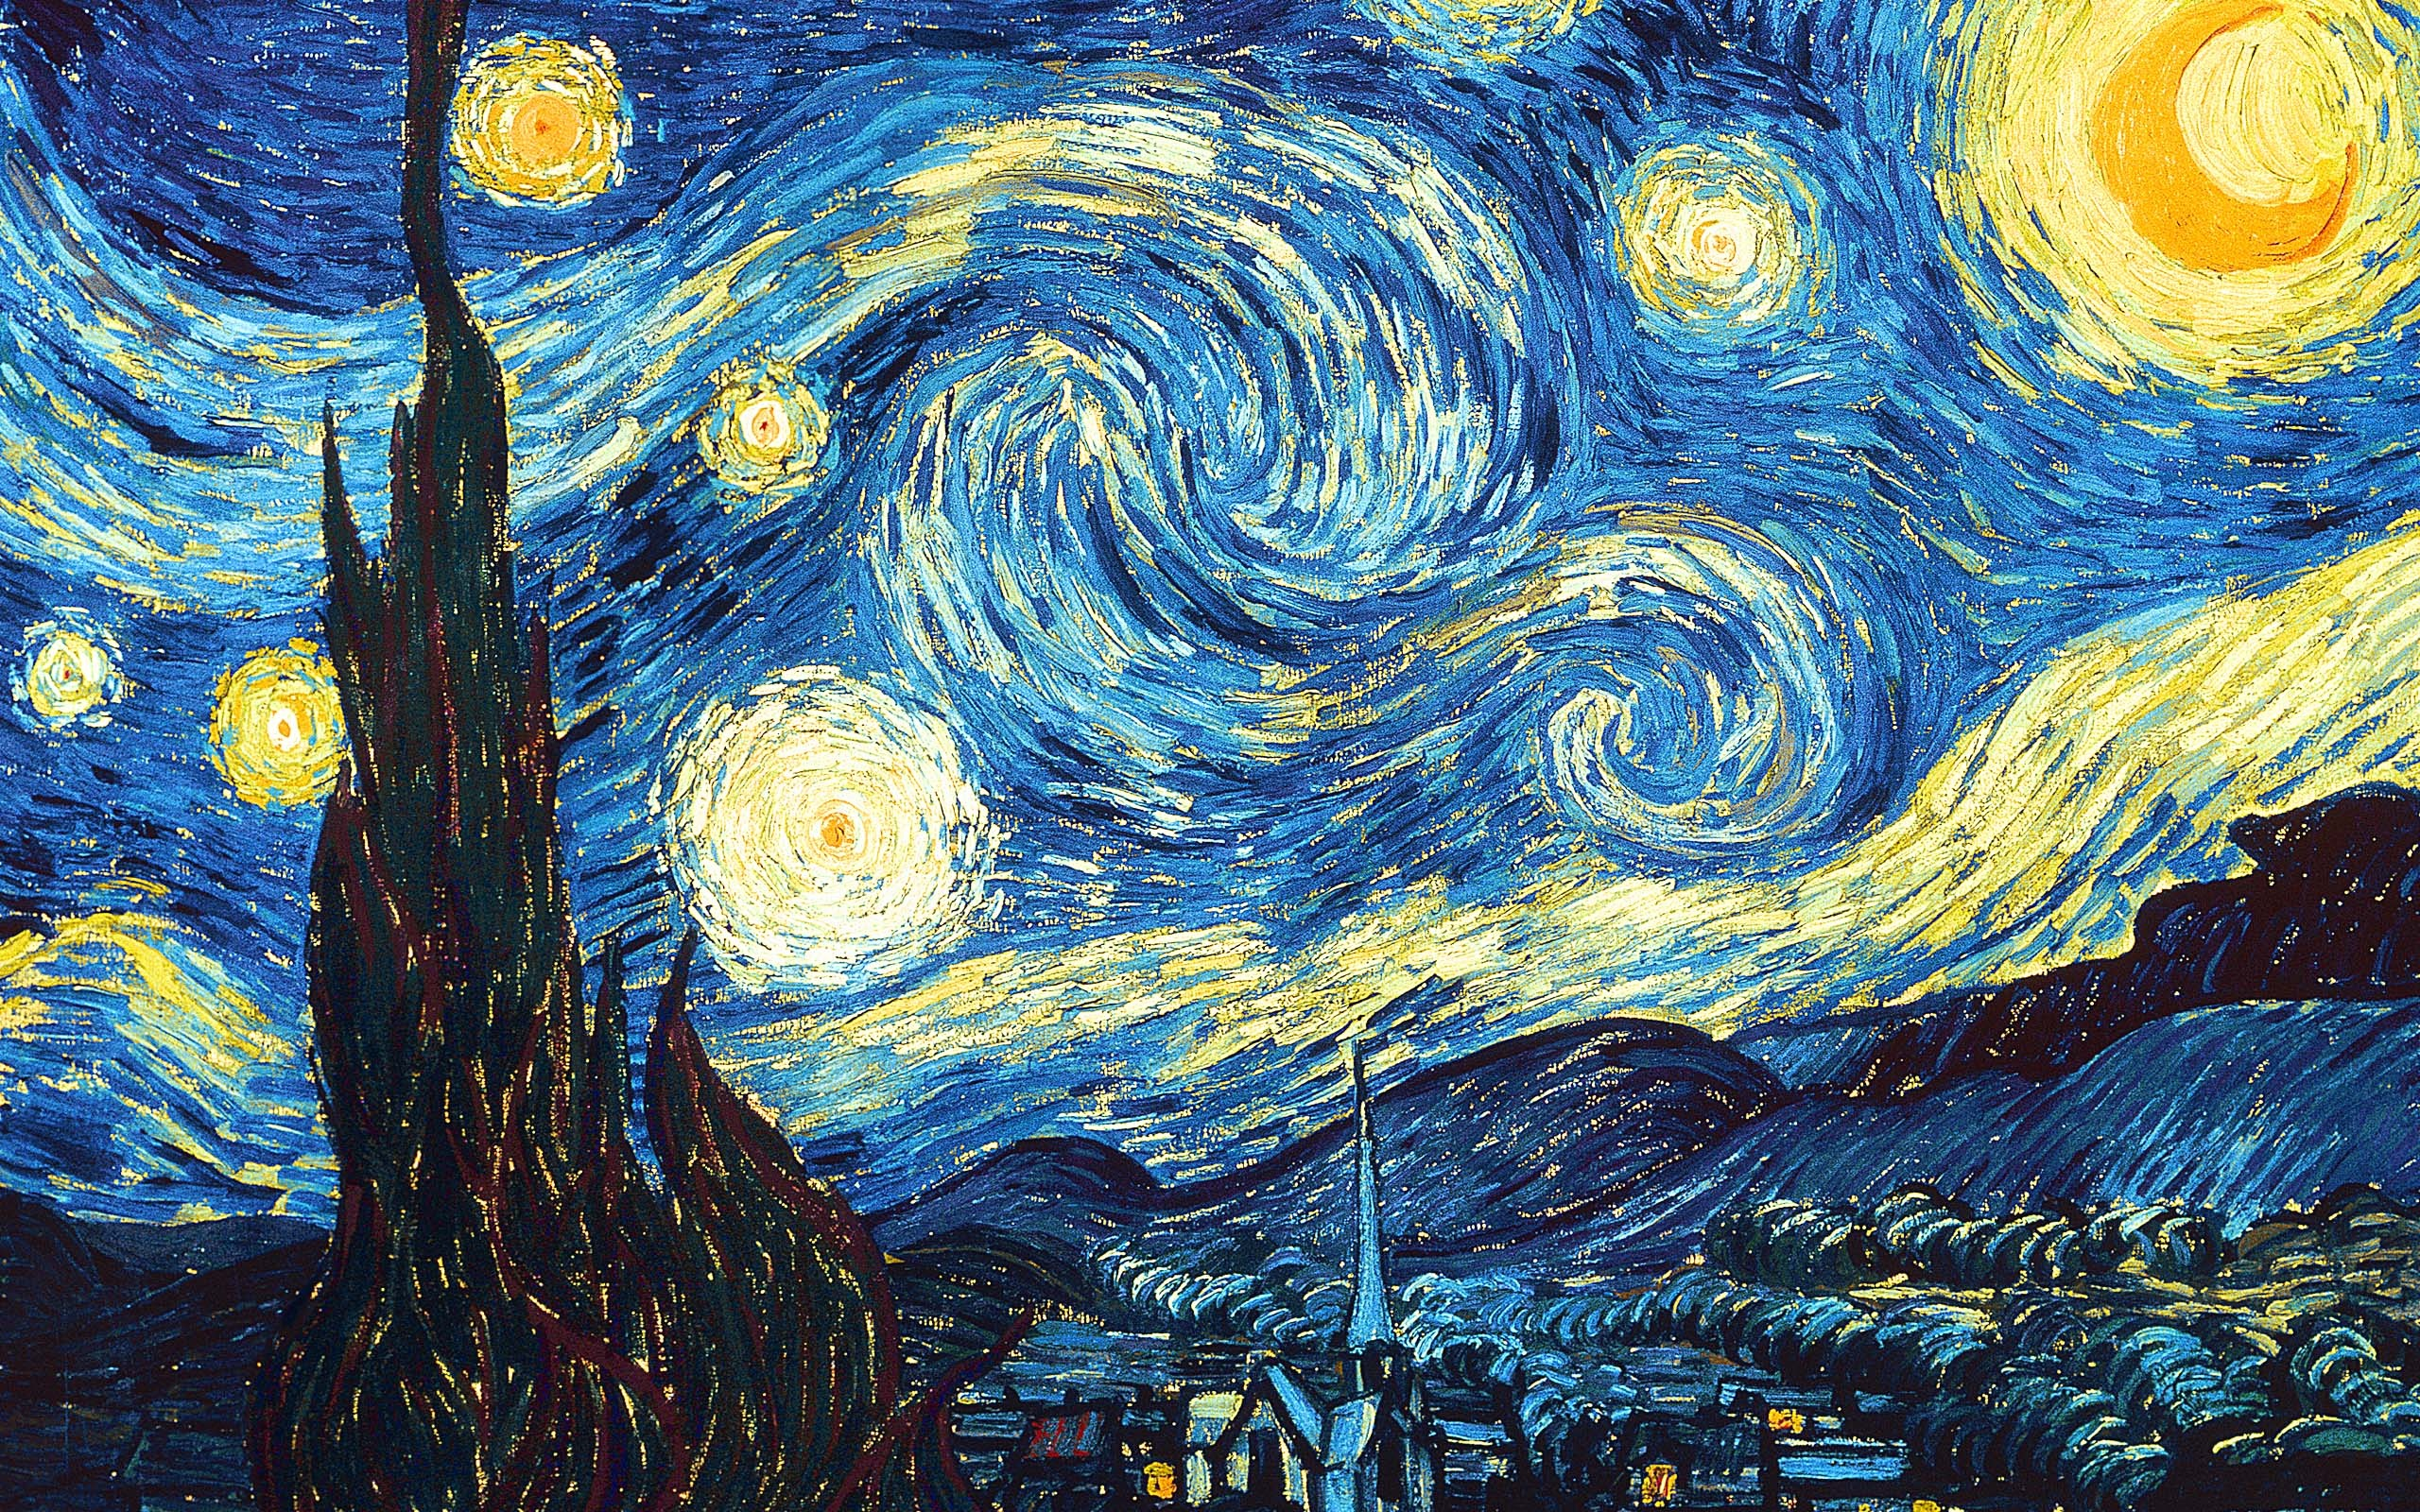
\includegraphics[scale=0.11]{the-starry-night-1889.jpg}
\end{figure}
\end{frame}

\begin{frame}{Cosa ci aspettiamo?}
\begin{figure}
\centering
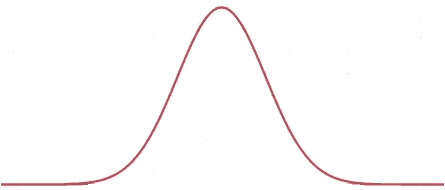
\includegraphics[scale=0.6]{gauss1.png}
\caption{Distribuzione \emph{gaussiana} }
\end{figure}
\end{frame}

\begin{frame}{Distribuzione di probabilità in \emph{Notte Stellata}}
\begin{figure}
\centering
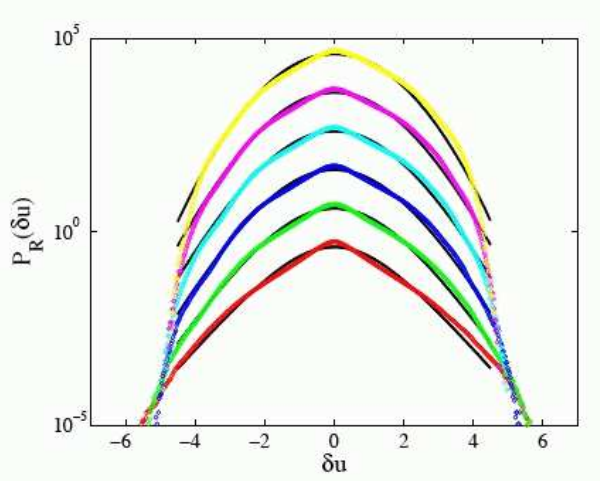
\includegraphics[scale=0.4]{gauss.png}
\end{figure}
\end{frame}

\begin{frame}{\emph{Campo di grano con volo di corvi}}
\begin{figure}
\centering
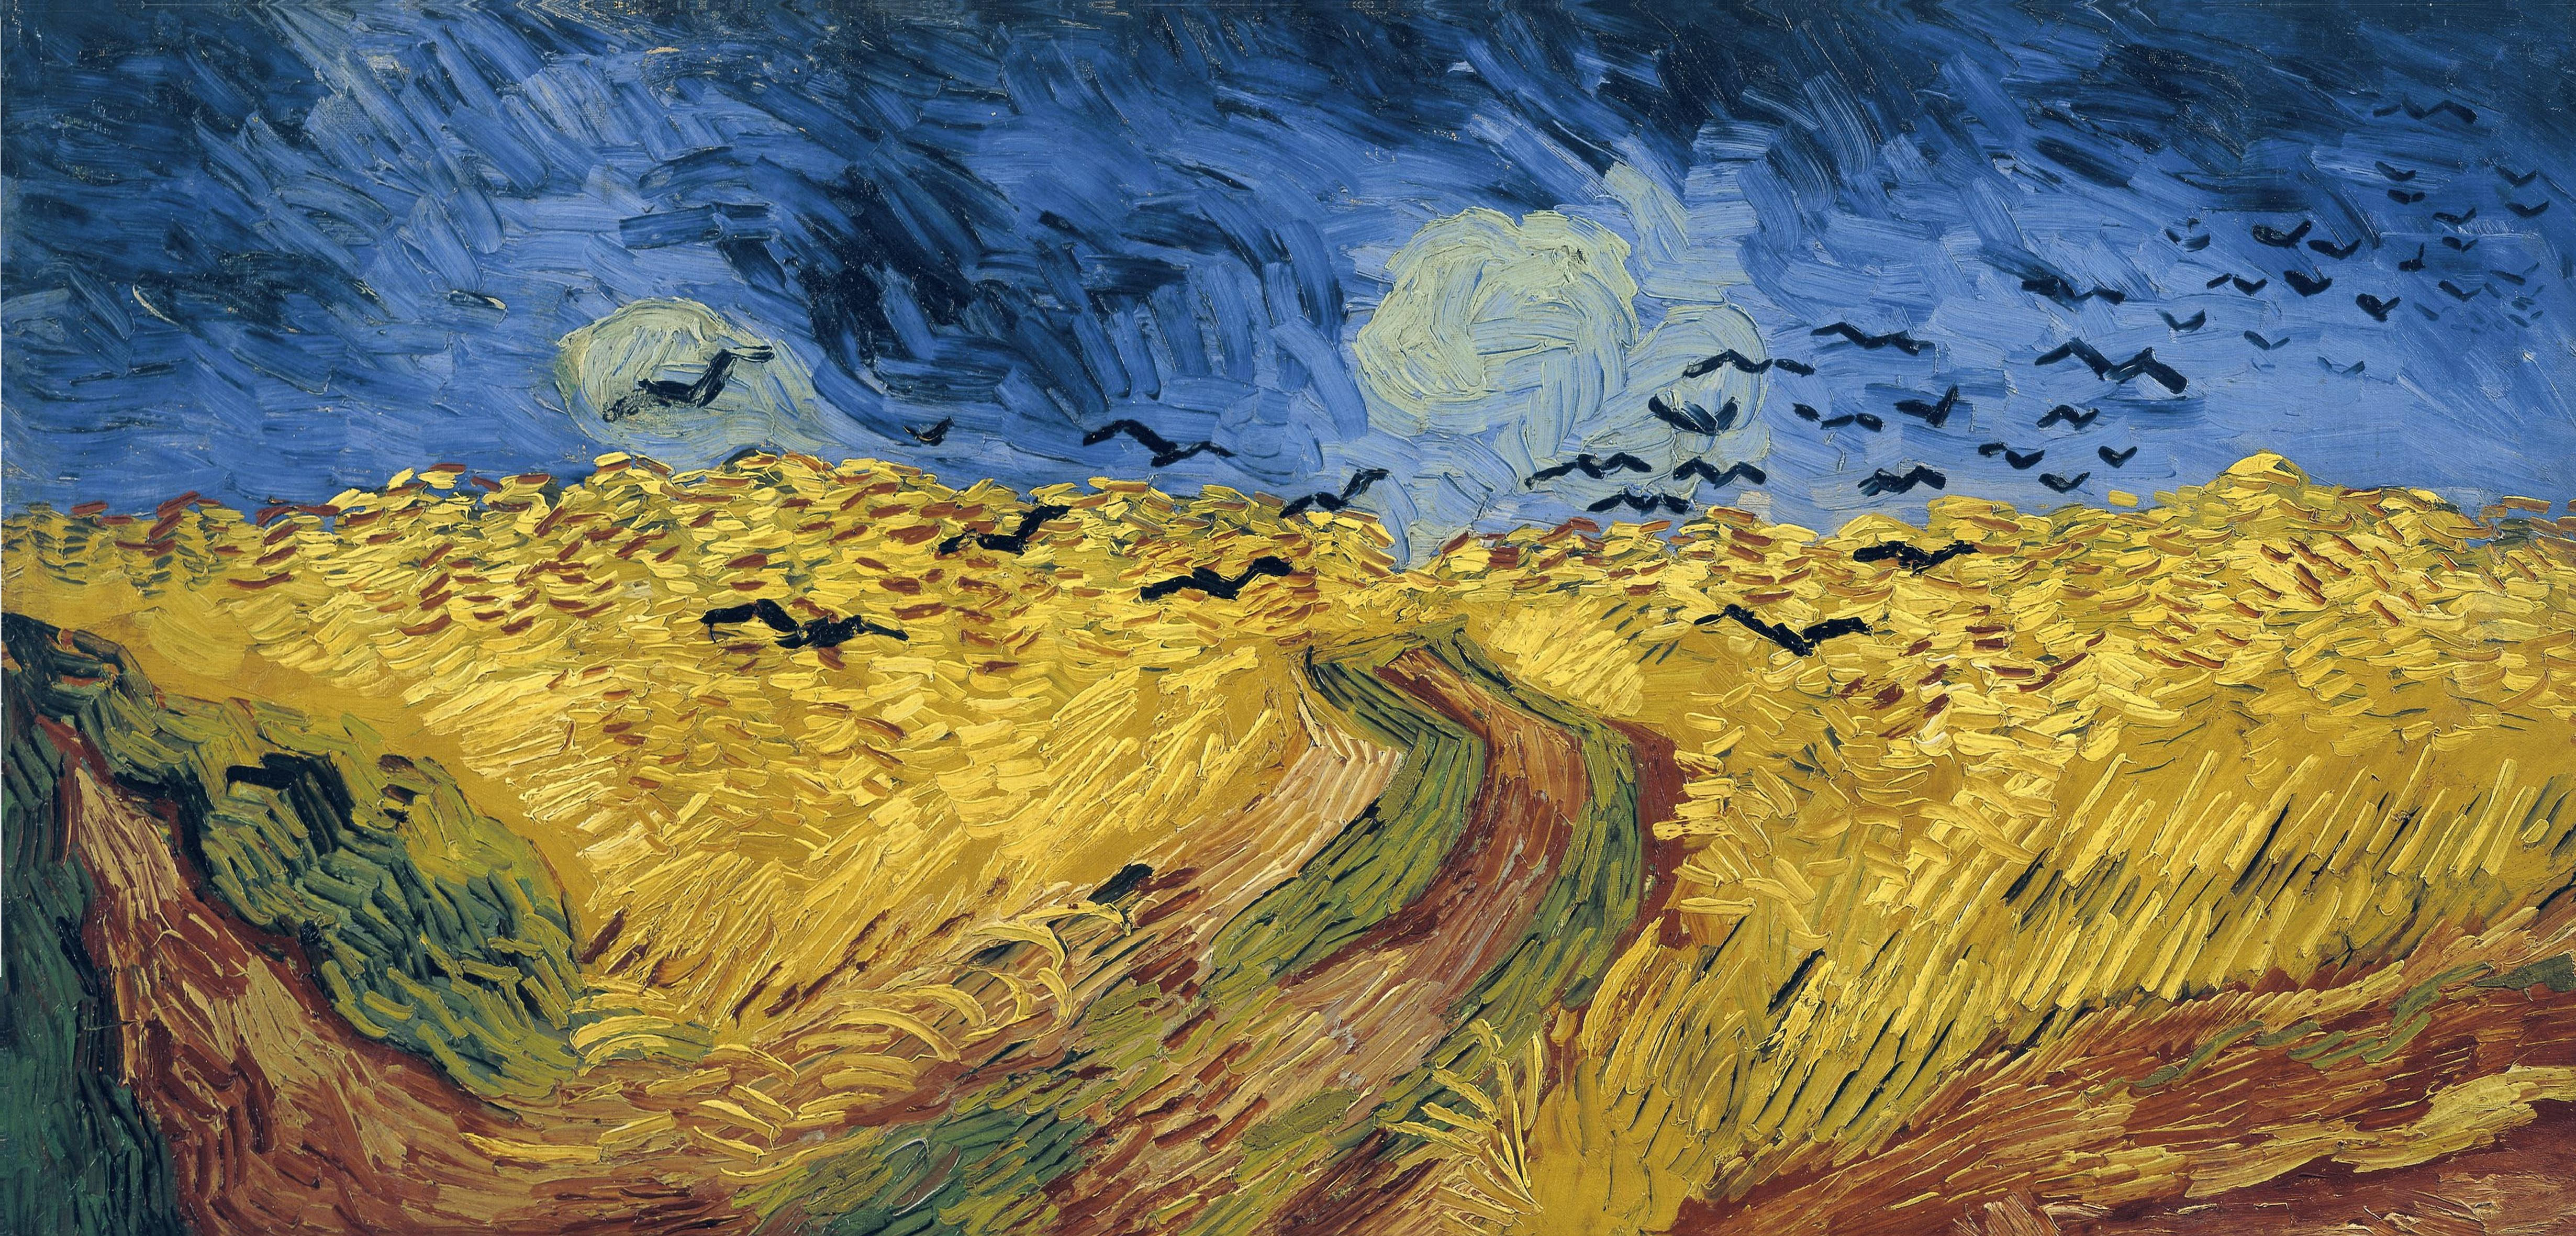
\includegraphics[scale=0.1]{wheatfield.jpg}
\end{figure}
\end{frame}

\begin{frame}{Distribuzione di probabilità nel \emph{Campo}}
\begin{figure}
\centering
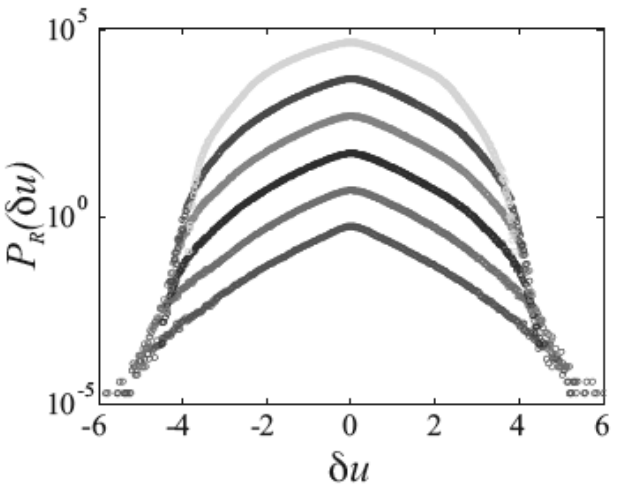
\includegraphics[scale=0.4]{PDF_wheat.png}
\end{figure}
\end{frame}

\begin{frame}{\emph{Strada e cipresso nella notte stellata}}
\begin{figure}
\centering
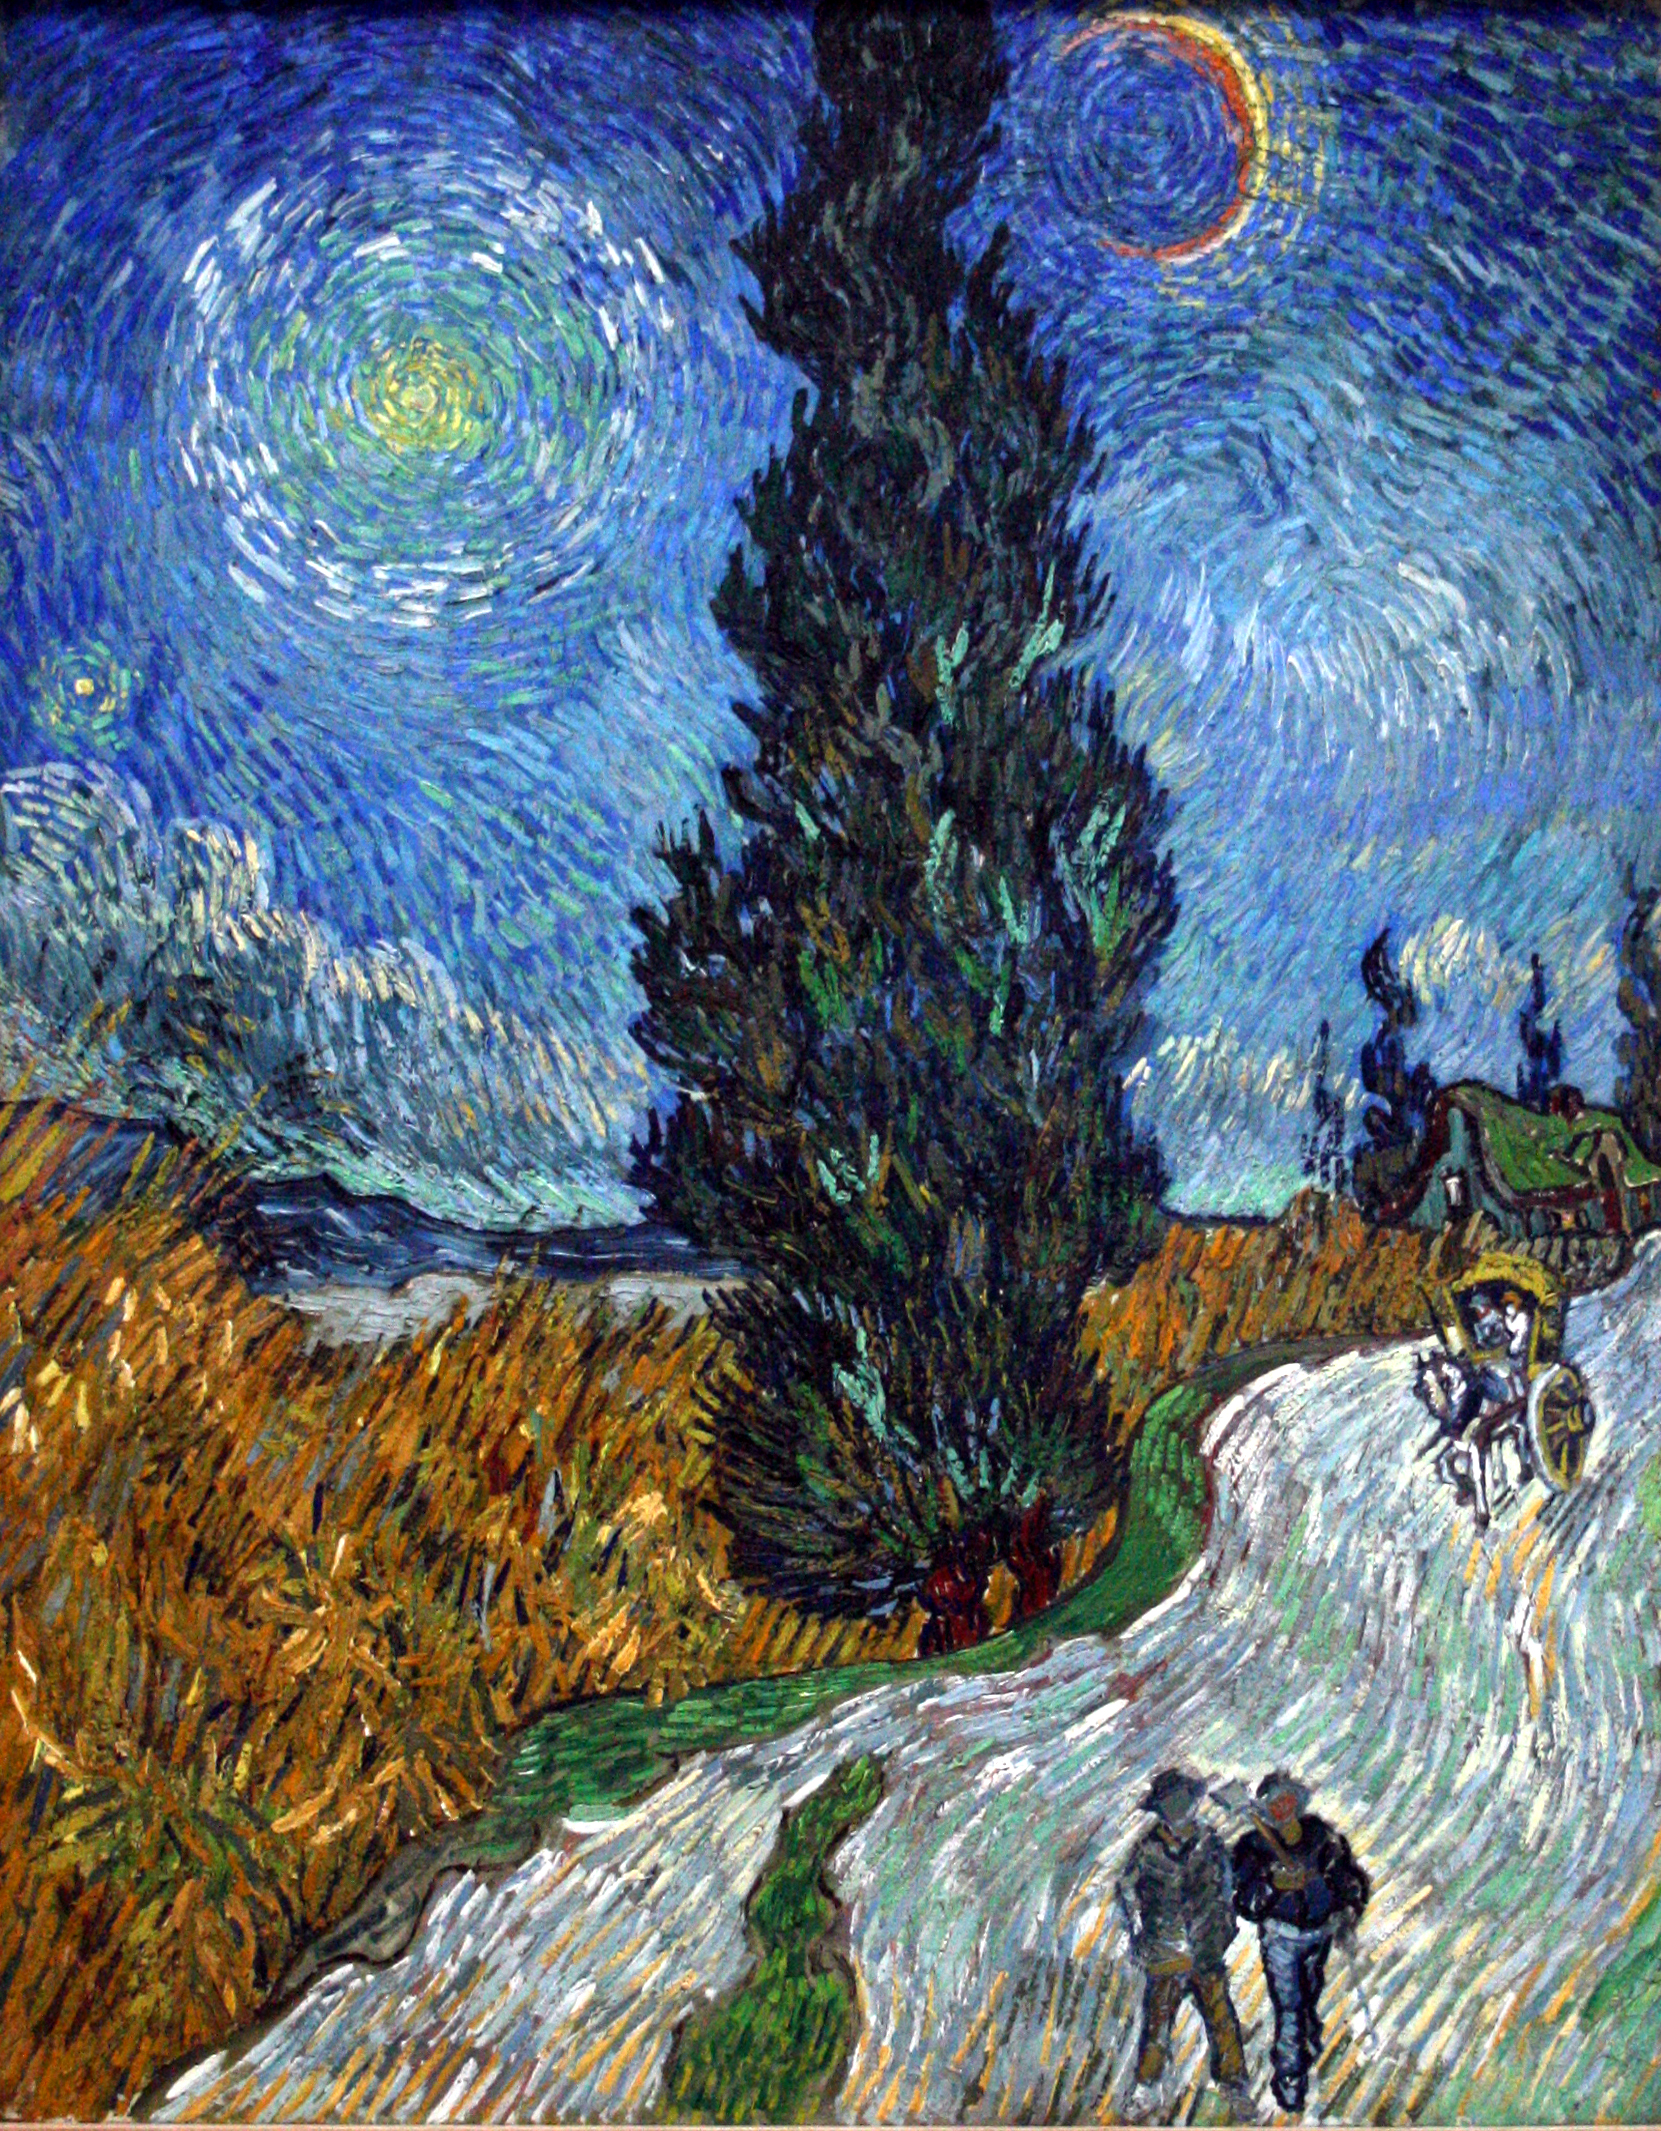
\includegraphics[scale=0.08]{road_cypress.jpg}
\end{figure}
\end{frame}

\begin{frame}{Distribuzione di probabilità nella \emph{Strada}}
\begin{figure}
\centering
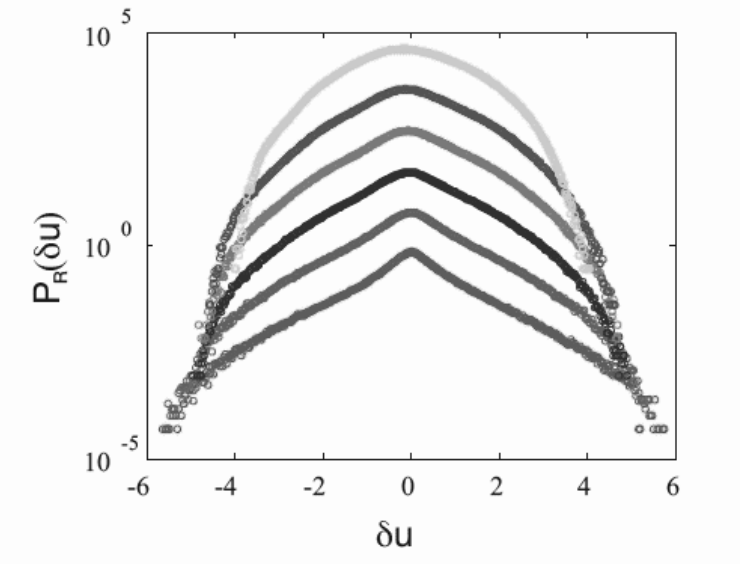
\includegraphics[scale=0.35]{PDF_road.png}
\end{figure}
\end{frame}

\begin{frame}{\emph{Autoritratto con pipa e orecchio bendato}}
\begin{figure}
\centering
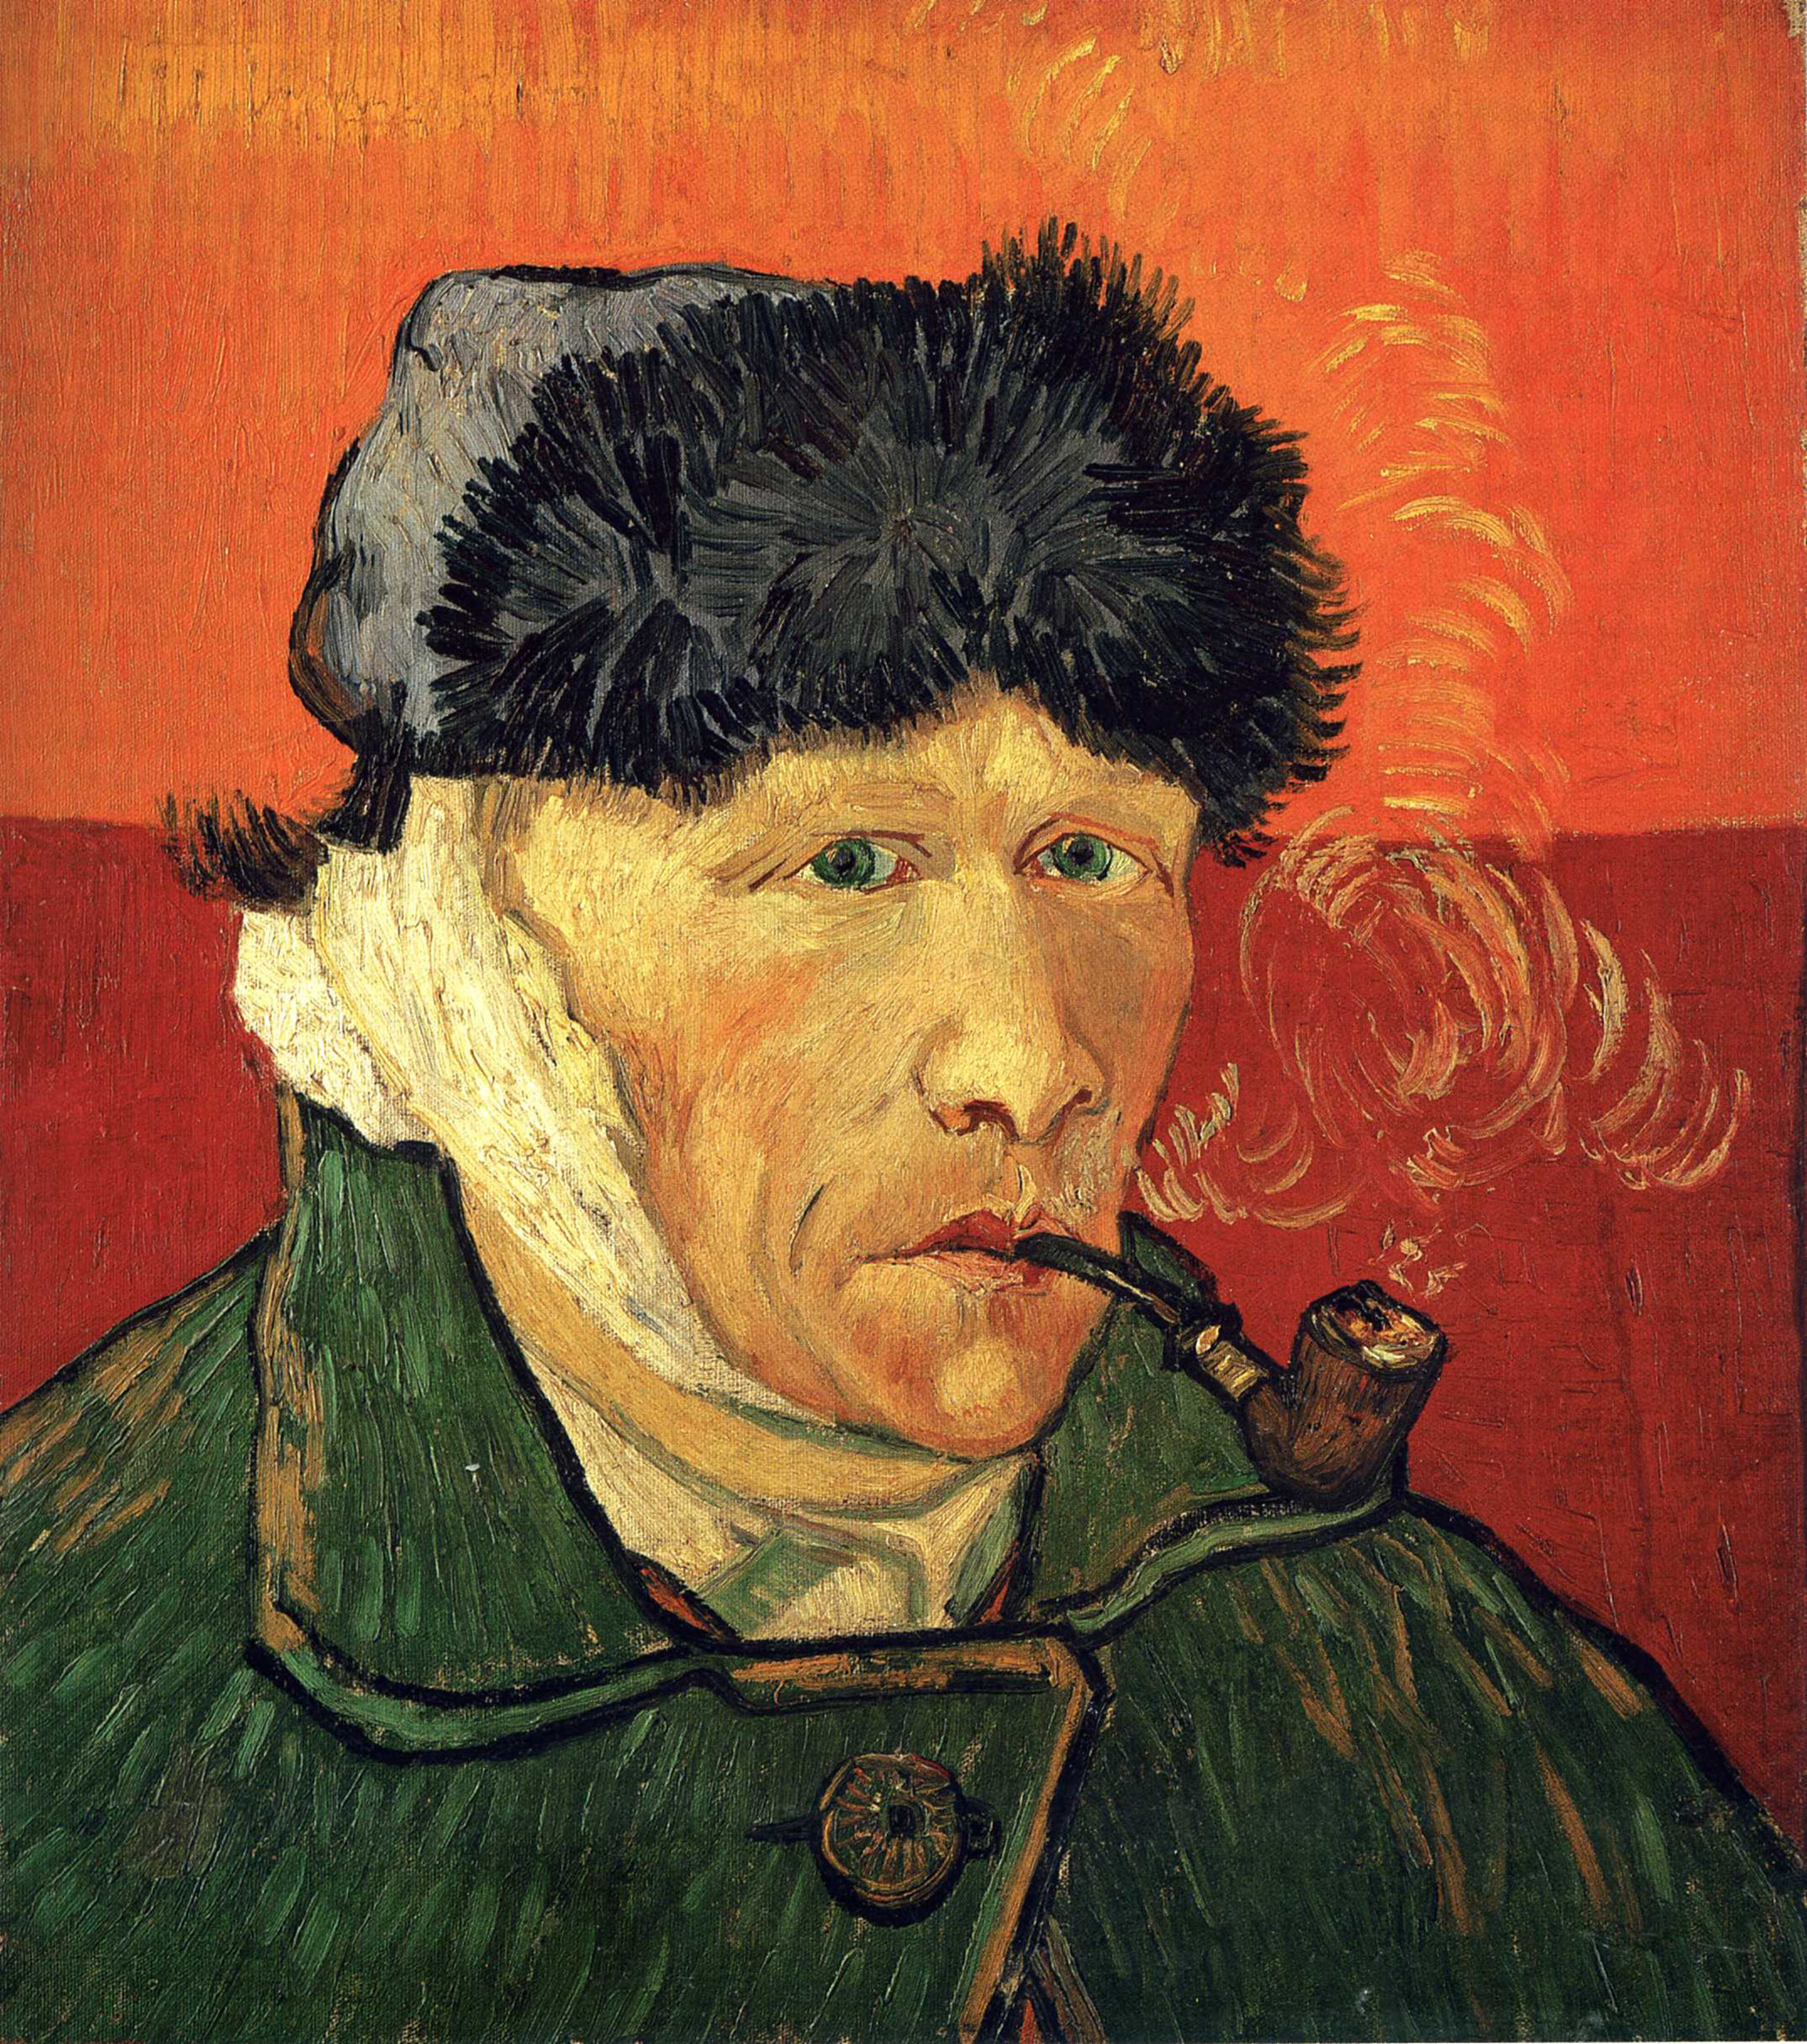
\includegraphics[scale=0.08]{selfportrait.jpg}
\end{figure}
\end{frame}

\begin{frame}{Distribuzione di probabilità nell'\emph{Autoritratto}}
\begin{figure}
\centering
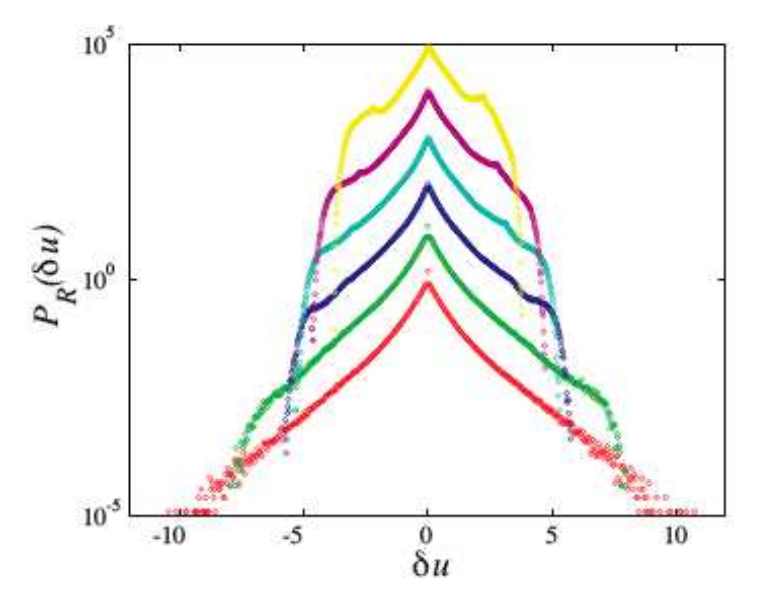
\includegraphics[scale=0.3]{PDF_self_portrait.png}
\end{figure}
\end{frame}

\section{La turbolenza in fluidodinamica}

\subsection{Il numero di Reynolds}

\begin{frame}{Il numero di Reynolds}
\begin{equation}
\text{Re} = \frac{\rho v L}{\mu} = \frac{\text{forze inerziali}}{\text{forze viscose}}
\end{equation}

dove $\rho$ è la densità del fluido, $v$ la velocità media del flusso, $L$ la lunghezza caratteristica del sistema, e $\mu$ il coefficiente di viscosità dinamica.
\end{frame}

\begin{frame}{Flusso a diversi numeri di Reynolds}
\begin{figure}
\centering
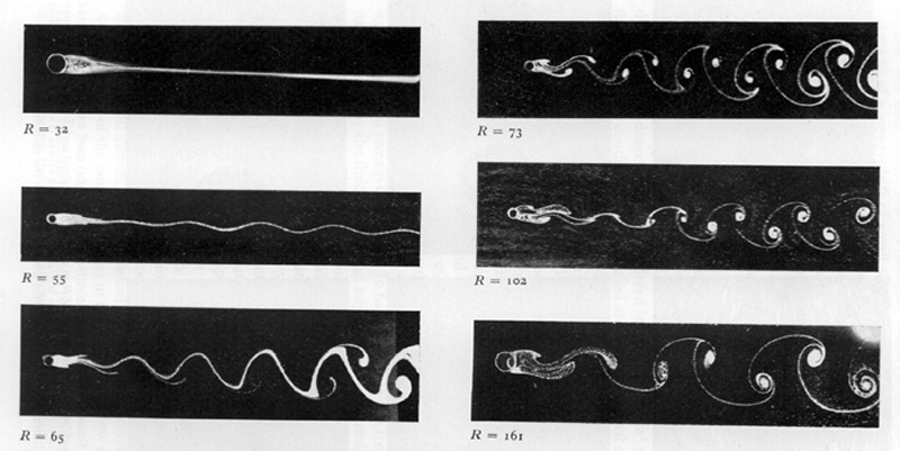
\includegraphics[scale=2.7]{allees.jpg}
\end{figure}
\end{frame}

\begin{frame}{Flusso a diversi numeri di Reynolds}
\begin{figure}
\centering
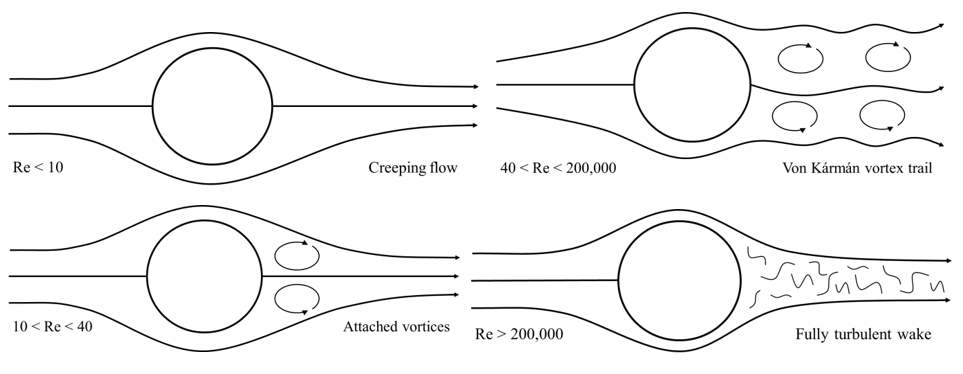
\includegraphics[scale=0.4]{flow_cylinder_6.png}
\end{figure}
\end{frame}

\begin{frame}{Il numero di Reynolds nel nuoto}
\begin{figure}
\centering
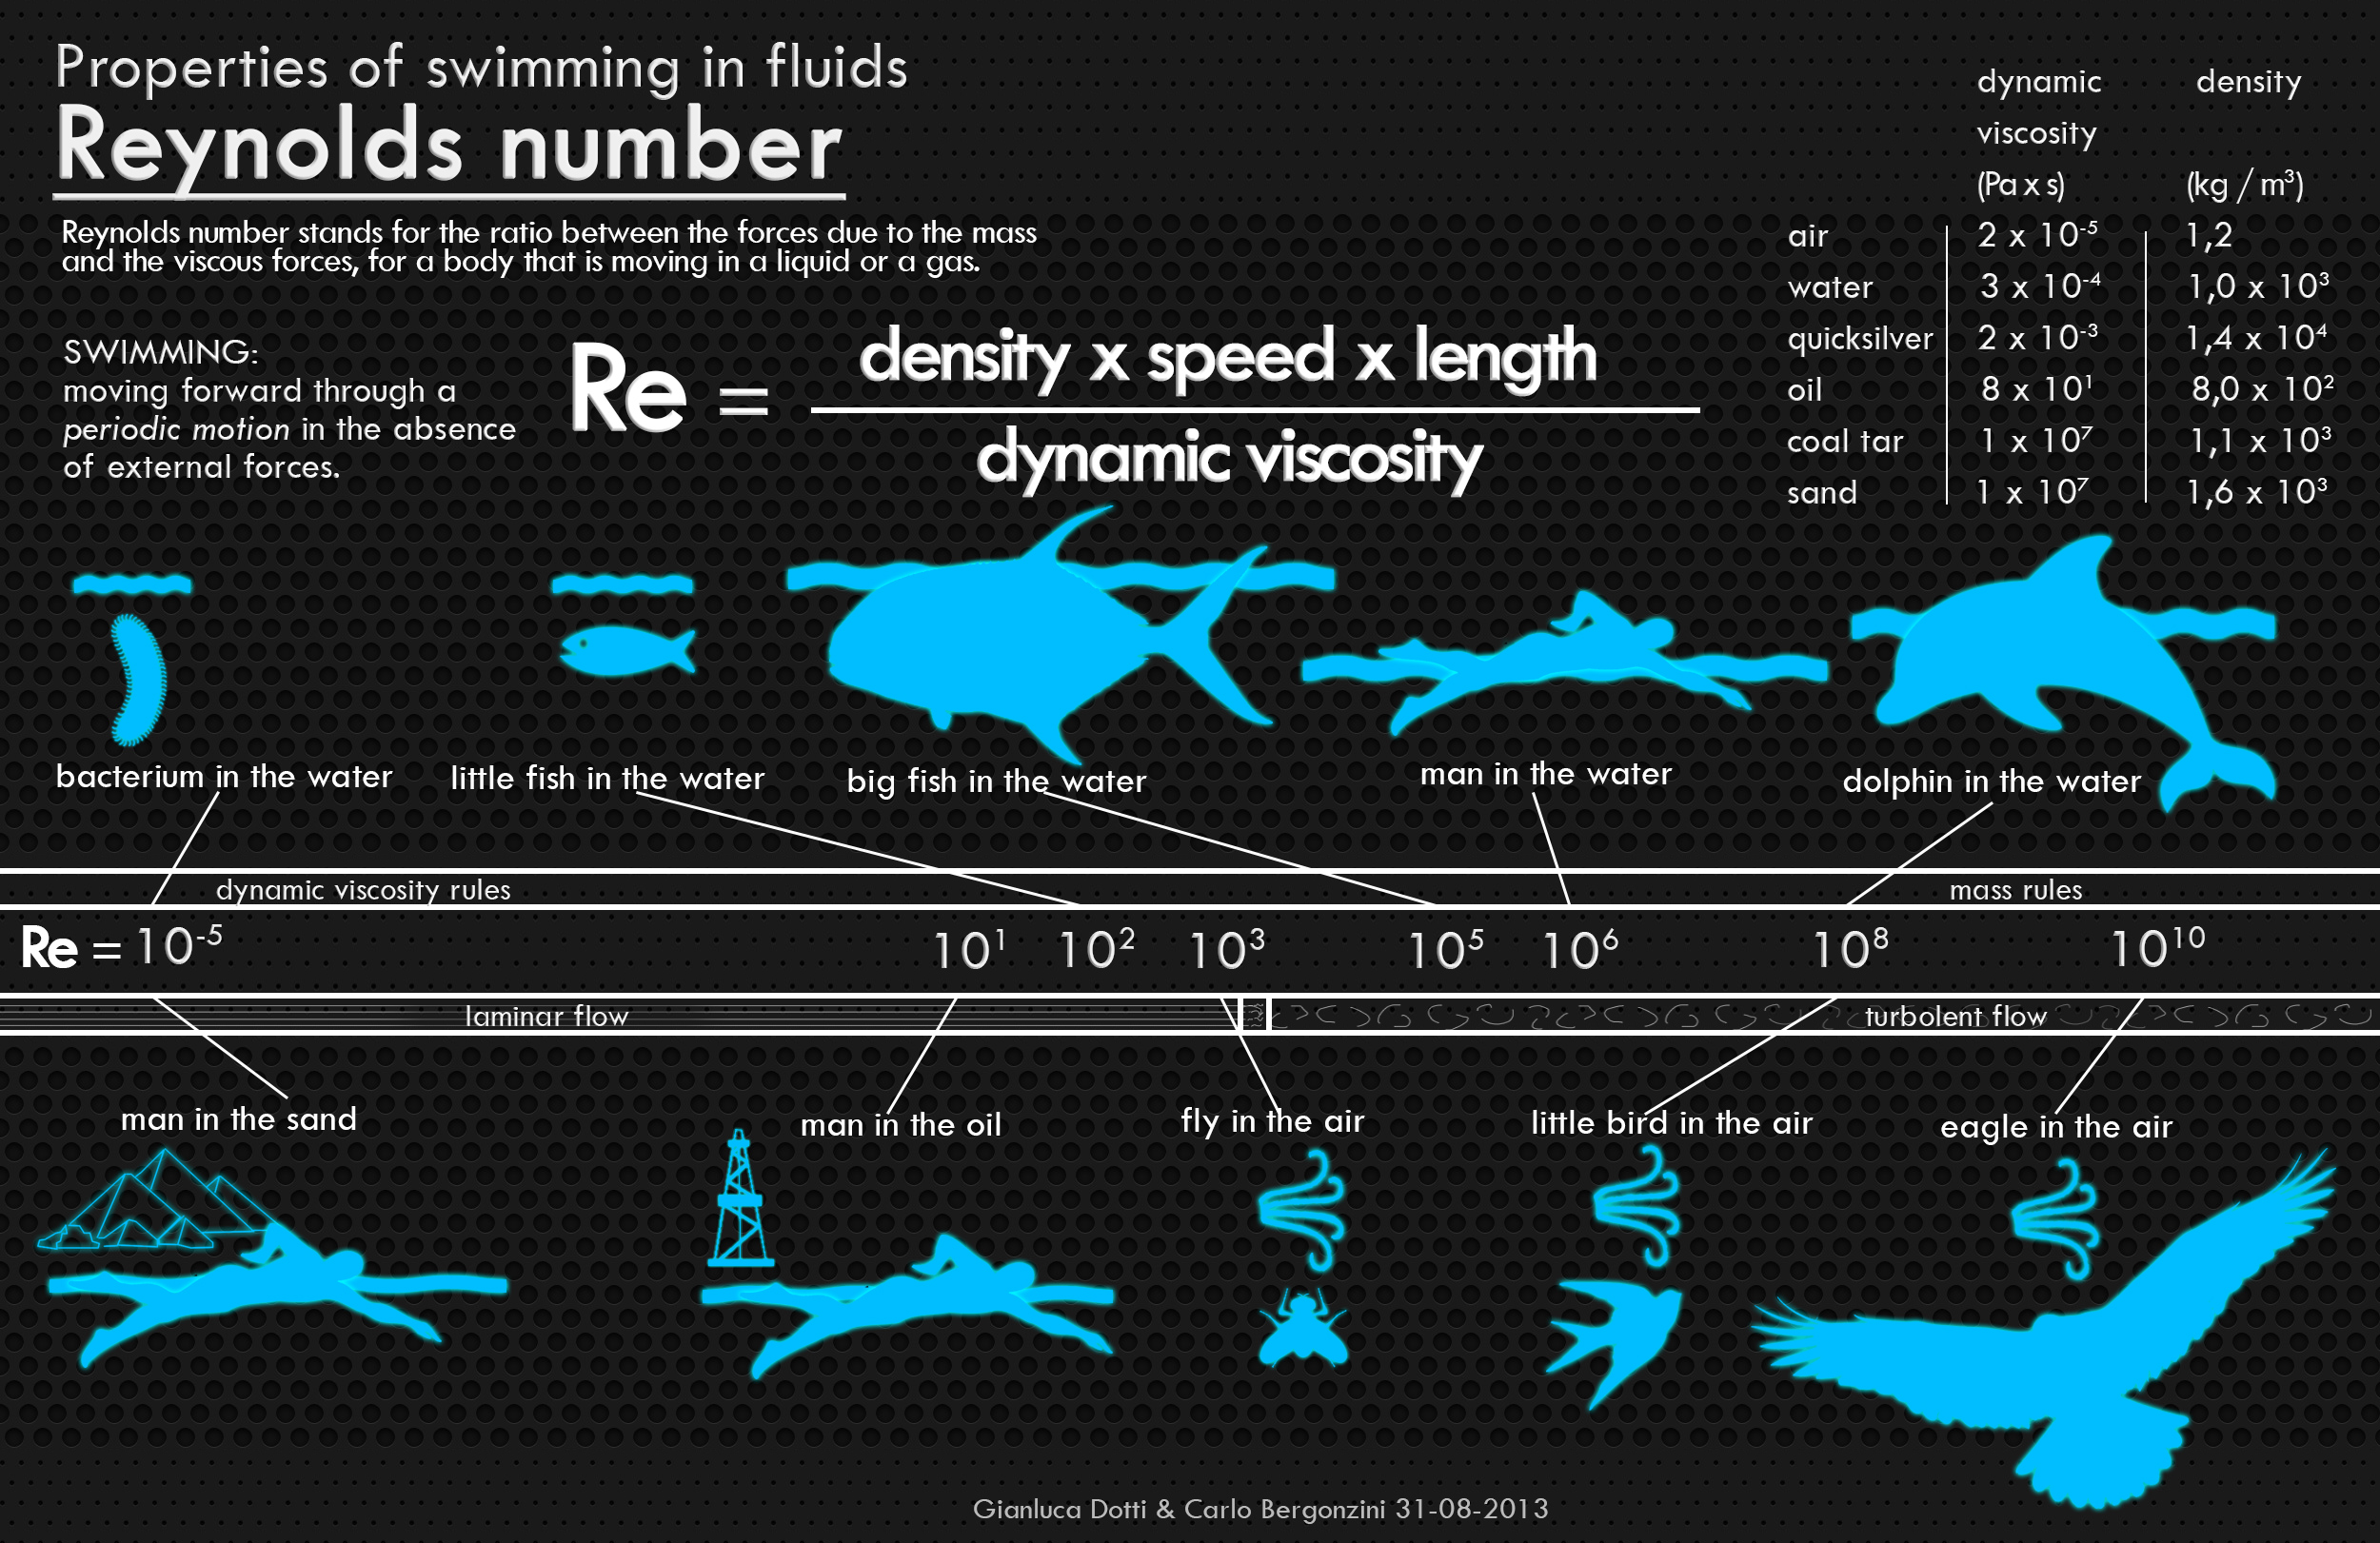
\includegraphics[scale=0.12]{infographic.jpg}
\end{figure}
\end{frame}

\subsection{Le equazioni di Navier-Stokes}

\begin{frame}{Ipotesi per le equazioni di Navier-Stokes}
\begin{itemize}
\item Densità del fluido costante (\emph{incompribimilità});
\item forza viscosa linermente dipendente da differenze di velocità (fluido newtoniano);
\item flusso isotropico;
\item assenza di forze esterne.
\end{itemize}
\end{frame}

\begin{frame}{Le equazioni di N.-S. in forma standard}
\begin{subequations}
\begin{align}
\frac{\partial \mathbf{v}}{\partial t} + \mathbf{v} \cdot (\nabla \mathbf{v})  &= -\frac{\nabla p}{\rho} + \nu \nabla^2 \mathbf{v} \label{navier-stokes} \\
\nabla \cdot \mathbf{v} &= 0
\end{align}
\end{subequations}

Significato:

\begin{itemize}
\item Termini a sinistra: derivata materiale;
\item termini a destra: forze sul fluido: gradiente di pressione e viscosità per il laplaciano della velocità (differenza fra la velocità in un punto e nei suoi dintorni);
\item seconda equazione: conservazione della massa per un fluido incomprimibile.
\end{itemize}
\end{frame}

\begin{frame}{Derivata materiale}

È la somma dell'accelerazione \emph{locale} (zero se il regime non cambia nel tempo) e di quella dovuta alla \emph{convezione}, ovvero quella dovuta dallo spostamento di particelle di fluido ad una parte diversa del flusso.

\begin{equation}
\frac{\dif \mathbf{v}}{\dif t} = 
\frac{\partial \mathbf{v}}{\partial t} \frac{\dif t}{\dif t} +
\frac{\partial \mathbf{v}}{\partial x} \frac{\dif x}{\dif t} +
\frac{\partial \mathbf{v}}{\partial y} \frac{\dif y}{\dif t} +
\frac{\partial \mathbf{v}}{\partial z} \frac{\dif z}{\dif t} =
\frac{\partial \mathbf{v}}{\partial t} + \mathbf{v} \cdot (\nabla \mathbf{v})
\end{equation}

(Immagine pompa pompiere)
\end{frame}

\begin{frame}{Le equazioni adimensionalizzate}
\begin{equation}
\frac{\partial \mathbf{v}}{\partial t} +\mathbf{v} \cdot (\nabla \mathbf{v}) = -\nabla p + \frac{1}{\text{Re}} \nabla^2 \mathbf{v}
\end{equation}

Il numero di Reynolds \emph{bilancia} le forze inerziali e quelle viscose.
\end{frame}

\subsection{La funzione di struttura}

\section{Il metodo dello studio}

\end{document}